
\section{Big picture}
 
Examining stimulus-response data and extrapolating from that a model
that allows us to predict, given a set of responses, what the stimulus 
likely was.


%---------This should be more general and give a big picture-------------
%----what do you want to accomplish?
%----what is neural activity in general?
%-----why is a low dim model important?
%-----is idea to understand how the brain is working?
%------How is the brain coding information?
%------how can we decode information based on brain activity?
%----what consequences would there be if we found a low dimensional structure?
%----what is the relevance of having a similarity measure?
%-----e.g want to know whether the brain is thinking about similar things 
%----at different brain states/instances
%----why?  --- what does this have to do with the structure of the space



\section{Biological background}
\subsection{Structure of a neuron}
A neuron is a specialized cell in the nervous system that receives, represents, and transmits information through a series of electrical pulses called action potentials or spikes. The action potentials are propagated at uniform strength and speed but with varying frequencies. The neuron is the fundamental unit of brain function. The neuron (see  figure \ref{fig:Neuron}) is made of three major parts, namely the dendrites (receive information from stimuli such as neurotransmitters), the cell body or soma (processes information) and the axon (transmits information to other neurons and other organs such as the brain).

\begin{figure}[h]
\caption{Structure of  a neuron}
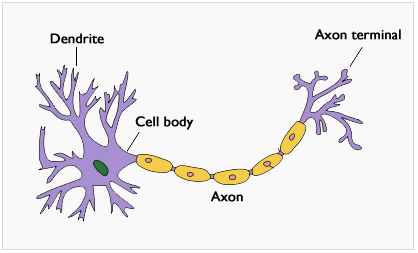
\includegraphics[width=\textwidth]{Neuron.jpg}
%label the figure so latex can reference it
      \label{fig:Neuron}
\end{figure}


The cell membrane is made up of phospholipids (fat) and separates the cell interior from the extracellular space. Embedded in the cell membrane are Na$^{+}$ (sodium) and K$^{+}$ (potassium) ion channels which pump out three Na$^{+}$ ions for every two K$^{+}$ ions pumped in. There are other ion channels (trans-membrane proteins) embedded in the cell membrane which
open or close (are gated)  enabling predominantly K$^{+}$, Na$^{+}$, Ca$^{2+}$ (calcium), and Cl$^{-}$ (chloride) ions to flow into and out of the cell. As a result, Na$^{+}$ is more concentrated outside the cell than inside it, and the intracellular concentration of K$^{+}$ is substantially higher than that outside the cell.
The lipid cell membrane is impermeable to charged ions but thin enough to allow interaction
of separated charged ions through electrostatic forces. 
Thus the cell membrane acts as an electrical capacitor whereas the gated ion channels act as conductors.

\subsection{Membrane potential}
A potential is a distribution of charge across the cell membrane.
\textit{Voltage} is a measure of the potential energy generated by separated charges and is measured in millivolts (mV). Ions flow into and out of the cell due to both voltage and concentration gradients. \textit{Current} refers to the flow of charged ions into and out of the cell. A resting neuron contains more negative charges on the inside than on the outside. 
This difference in separated charges is called the neuron's \textit{membrane potential}
whose value is represented by charge in the intracellular space relative to that in the extracellular fluid. A neuron with a negative membrane potential of approximately -70mV is called \textit{polarized}. This number is also referred to as the resting membrane potential.
In a resting neuron, all the voltage-gated ion channels are closed. 

\subsection{Generation of an action potential}
Dendrites contain chemically-gated Na$^{+}$ channels which open when 
a stimulus affects a sensory receptor, such as neurotransmitters binding to the dendrite receptors. This leads an influx of Na$^{+}$ into the intracellular fluid, causing the membrane potential to be less negative or positive (depolarization of the neuron). 
This increase in the membrane potential causes  the voltage-gated Na$^{+}$ channels, at the axon hillock, to open and more Na$^{+}$ flows into the cell down its electrochemical  gradient. When a certain threshold is reached ($\approx$ -55mV), an electrical pulse lasting  a short duration ($\approx$ 1ms),  called an \textit{action potential}, is released and propagates long distances along the neuron's axon. When the membrane potential rises (to  $\approx$ 40mV), the voltage-gated K$^{+}$ channels open and more K$^{+}$ flows out of the cell causing
the membrane potential to fall below the resting potential (hyperpolarization of the neuron).
The neuron later returns to it's resting potential after a refractory period.
\textit{A refractory period} refers to a period where the spiking probability of the cell is greatly reduced immediately following the release of an action potential.
The opening of voltage-gated ion channels at one point on the axon
activates nearby gated-channels (along the nodes of ranvier) resulting into a wave of action potentials down the the axon terminal. The axon terminal contains voltage-gated Ca$^{2+}$ channels which open and release neurotransmitters into the synaptic cleft. The neurotransmitters bind onto the dendrite receptors of nearby neurons.
A synapse is a means by which different neurons communicate. The neuron which sends off an action potential is called a \textit{presynaptic neuron} and the neuron which receives the 
chemical message is called a \textit{postsynaptic neuron}.
An action potential which results into excitation of a postsynaptic neuron is called an 
\textit{excitatory post synaptic potential} (EPSP) while that resulting into inhibition of a postsynaptic neuron is called an \textit{inhibitory post synaptic potential} (IPSP). 


\subsection{Measuring Neurons.}
An \textit{electrode} is an object  which allows electric current to pass through it
and is used to make contact with an electrolyte during the study of electrical properties
of biological cells (electrophysiology). 
A very small electrode is called a \textit{microelectrode} while a large electrode
is called a \textit{macroelectrode}.
Macroelectrodes are used to measure simultaneous electrical activity of neuronal populations
either on the surface of the scalp (electroencephalogram or EEG) or on the surface of the cortex (electrocorticogram or ECoG). Microelectrodes are typically used to measure 
single unit spiking activity or stimulation of nerve cells.
A \textit{single unit} refers to a single, action potential generating neuron, whose spikes are clearly isolated by a recording microelectrode. (cite the reference for this and next figure).
The \textit{local field potential} (LFP) refers to the sum of numerous extracellular potentials
generated by flow of ionic currents across the cell membrane, distributed along multiple neurons, due to the discharge of an action potential from a presynaptic neuron.
LFPs represent summed average synaptic potentials in a given volume of the brain and can
be used to characterize synaptic inputs as either excitatory or inhibitory.
Membrane potentials are measured using \textit{intracellular recordings}, a process where an electrode (such as a hollow glass electrode filled with conducting electrolyte) is inserted inside the cell body. The value of the membrane potential is obtained by comparing the potential on the inserted electrode to that of a reference electrode placed in the extracellular fluid surrounding the cell body.  The process in which an electrode is inserted in the extracellular space near the cell body is called \textit{extracellular recording} (see figure  \ref{fig:Electrodes}).

\begin{figure}[h]
\caption{Macroelectrodes Vs Microelectrodes}
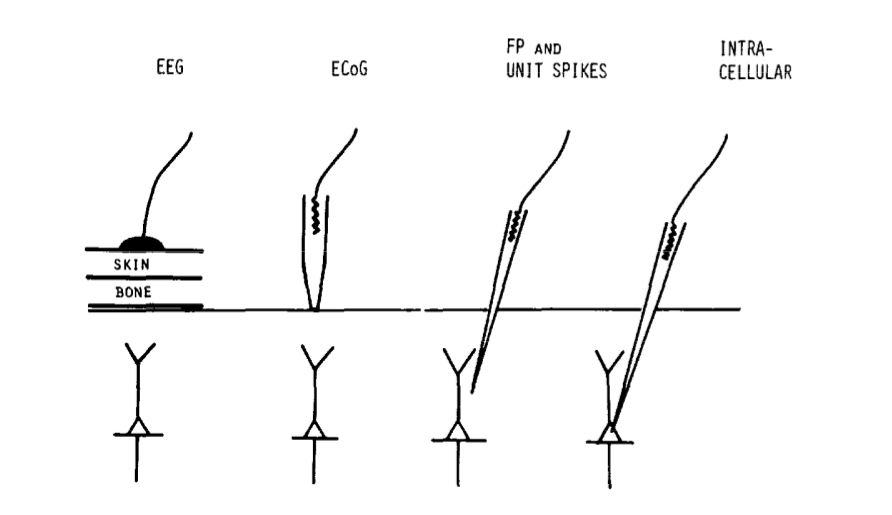
\includegraphics[width=\textwidth]{Electrodes.png}
%label the figure so latex can reference it
      \label{fig:Electrodes}
\end{figure}

Both extracellular and intracellular recordings are used to record potential due to synaptic transmissions (LFPs) and potential due to firing of an action potential.
Intracellular recordings enable visualization of the cell structure and identification
of the cell type by adding a dye inside the electrolyte contained in the glass electrodes.
Extracellular recording are usually carried out in living brains (in vivo) or behaving animals
while intracellular recordings can be carried out both in vivo and also in vivtro preparations, such as slices of brain tissue. Multi-electrode arrays such as the $10 \times 10$ utah array (cite the professor who designed it)  enable simultaneous extracellular recordings from  multiple neurons in multiple brain sites. 
Intracellular recordings for instance in behaving animals such as rats may be carried out using 
a collection of tetrodes (cite Recce and O'keefe).
A tetrode is a bundle of 4 individually insulated fine wire electrodes. In both cases, potentials are recorded at the tip of each electrode. 



Multi-unit single-trial recordings refer to simultaneous  extracellular recordings of neural activity from hundreds of cells.
For Spike Train analyses, the multi-unit single-trial recordings are usually processed using  Spike sorting methods  based on  either amplitude and wave form variation or on spatial location. After which, neuronal types are identified by classifying the isolated units into known cell groups of the cortex.

The data set we are analyzing is based on intracellular multiple single-unit single-trial recordings where the action potentials are measured from different cell membranes using tetrodes. Tetrodes are used in the rat hippocampus where there is a dense network of cells which would otherwise be hard to isolate using the usual spike sorting methods as in multi-unit single-trial recordings.


\subsection{Place cells}


\subsection{Place fields}


\subsection{Characteristics of place fields}





\newpage


















































%=========================================================================================


%=======Below was my original objective===================================================
%The objective of this present project is to find a low dimensional model of interactions, among a subtype of neurons called place cells, in the CA1 region of the rat hippocampus, believed to be specified to relay the animal's physical position. The model is extrapolated from application of a non-linear dimensionality tool called diffusion maps, to a designed 
%similarity matrix of activity patterns.\\



%======================Gaussian Processes below for future works==============================
%\newpage
%\section{Linear dimensionality reduction techniques}
%\subsection{Gaussian Process Factor analysis}
%\begin{Def}
%A vector-valued random variable $\vect{X} = \left[x_{1}, \ldots , x_{n} \right]^T$
%has a multivariate Gaussian distribution if it's  probability density function is given by
%   
%\[
%f(\vect{x})  = (2\pi)^{-\frac{n}{2}} \det({\Sigma})^{-\frac{1}{2}} 
%\exp \bigg( -\frac{1}{2}(\vect{x - \mu})^{T}\Sigma^{-1}(\vect{x - \mu}) \bigg)
%\]
%
%with mean vector  $\vect{\mu} \in \mathbb{R}^n$ and covariance matrix $\Sigma$.
%The covariance matrix must be a positive semidefinite (PSD) matrix for such a density to exist.
%We write $X  \sim N(\vect{\mu}, \Sigma).$
%
%\end{Def}
%
%
%\begin{Def} A Gaussian Process (GP) is a Gaussian distribution over functions \\
%$f: \mathbb{R}^n \rightarrow   \mathbb{R}^n$  defined by specifying a mean
%function $m: \mathbb{R}^n \rightarrow \mathbb{R}$  and a kernel
%$K: \mathbb{R}^n  \times \mathbb{R}^n \rightarrow \mathbb{R} $ such that the following
%conditions hold:
%
%\begin{itemize}
%\item each vector valued random variable 
%$f(\vect{t}) = \left[f(t_1), \ldots , f(t_n) \right]^T$ has a multivariate Gaussian distribution for all  
%$\vect{t} = \left[t_1, \ldots, t_n   \right]^T$, that is, 
%$f(\vect{t}) \sim  N(m(\vect{t}), K(\vect{t}, \vect{t})).$
%
%\item $m(\vect{t}) = \E(f(\vect{t}))$
%
%\item $K(\vect{t},\vect{s}) = \E\left[ \big(f(\vect{t}) - m(\vect{t}) \big) \big( (f(\vect{s}) - m(\vect{s}) \big)^T   \right]$  for any $\vect{t}, \vect{s} \in \R^n.$  
%
%\item K satisfies the Mercer theorem.
%
%\end{itemize}
%\end{Def}
%
%\begin{Thm}
%
%Every matrix $ K(\vect{t}, \vect{t}) = \{ K(t_i, t_j) \}_{1 \leq i, j \leq n} = (k_{ij}) $
%is a PSD  for all time $\vect{t}$ if
%\[  \vect{v}^T K \vect{v} = 
%\sum_{i=1}^{n} \sum_{j=1}^{n} k_{ij} v_i v_j =
% \sum_{i=1}^{n} \sum_{j=1}^{n} k(t_i, t_j) v_i v_j \geq 0  
% \quad \text{for all}  \quad \vect{v}  \neq \vect{0}. \] 
%
%\end{Thm}
%
%
%\begin{Ex}
%One of the most commonly used kernels is the squared exponential kernel (SE) given by
%$K(t_{i}, t_{j}) = \sigma_{f}^{2} \exp \{-\frac{1}{2l^2}  (t_i - t_j)^2 \}$
%where $\sigma_{f}^{2}$  is the variance of the kernel and l is the length scale.
%
%\end{Ex}
%



%============================================================================================
%%======How to insert a table in latex===================%

%\begin{table}[H]
%   \centering
%    \begin{tabular}{|c|c|c|c|}\hline
%    $x$ & 0 & 1 & 2\\ \hline
%    $f(x)$ & 3 & 6 & 9\\ \hline
%    \end{tabular}
%     \caption{Caption goes here}
%\end{table}

%%=====end table==================================%
%\begin{figure}[H]
%  \centering
%    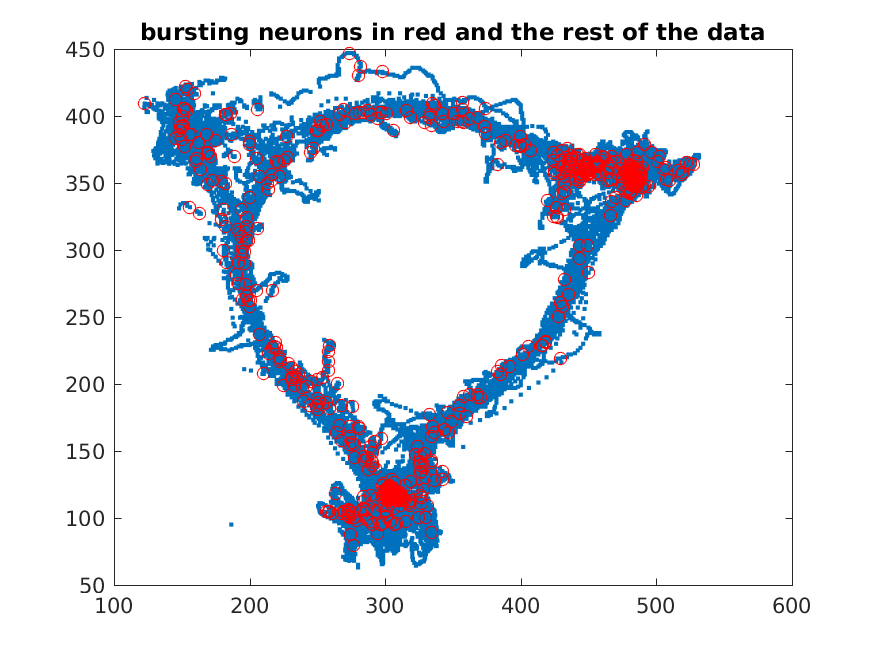
\includegraphics[scale=0.5]{Bursting_neuron.png}
%     \caption{The bursting neuron}
%      \label{tab:data1}
%\end{figure}


%===========Insert a figure in latex=============%






%============end figure===========================%

%\begin{itemize}
%\item What is the nature of the problem you're trying to solve?
%\item Two most well known models that inspired your work
%\item The authors and names of these models
%\item What were they modeling?
%\item Strengths and weaknesses of these models
%\item Overview of our model
%\item What is promising about our model
%\item why are you going to use dimensionality reduction to study the model
%\item why use vector space embeddings instead of the point process framework
%\item Report any results that may be significant and supported by a measure of "goodness"
%\item Mention that this is the first time this type
%of analysis has been applied to the Redish Lab data 
%obtained from the CA1 region of the Hippocampus
%\end{itemize}

